\chapter{Implementacja}

\section{Architektura}

Diagram \ref{fig:architektura} przedstawia architekturę aplikacji wraz z jej osadzeniem w potencjalnym środowisku uruchomieniowym.

Aplikacja składa się z 3 modułów:

\begin{itemize}
	\item Systemu udostępniającego zadania do wykonania. 
	Jego zadaniem jest generowanie, zlecanie oraz prezentowanie uzyskanych wyników planowania.
	\item Systemu odbierającego zadania planowania i przekazującego żądania do węzłów obliczeniowych.
	\item Węzła obliczeniowego wykonującego planowanie przy pomocy wybranych algorytmów. 
	Jego zadaniem jest wykonanie planowania według zadanych parametrów, zebranie informacji związanych z efektywnością (np. czas wykonania, ilość wykorzystywanej pamięci etc.) wybranego algorytmu, oraz zwrócenie wyników do zlecającego klienta.
\end{itemize}

W ramach konkretyzowania modelu przedstawionego w koncepcji na rysunku \ref{fig:wizja} zdecydowaliśmy się wykorzystać SOAP WebService w celu przyjmowania zadań od klientów.
Po stronie naszej referencyjnej implementacji klienta zdecydowaliśmy się wykorzystac REST WebService w celu odbierania wyników planowania.
W sekcji \ref{sec:webservices} przedstawiamy krótką motywację tej decyzji.
Dodatkowo zdecydowaliśmy się na konkretną reprezentację zadań planowania oraz ich parametrów - postanowiliśmy wykorzystać reprezentację GEXF, a także na reprezentację wyników.
Obie te reprezenatcje oraz motywację dla tej decyzji przedstawiliśmy w sekcji \ref{sec:data}.

\begin{figure}[!h]
	\centering
	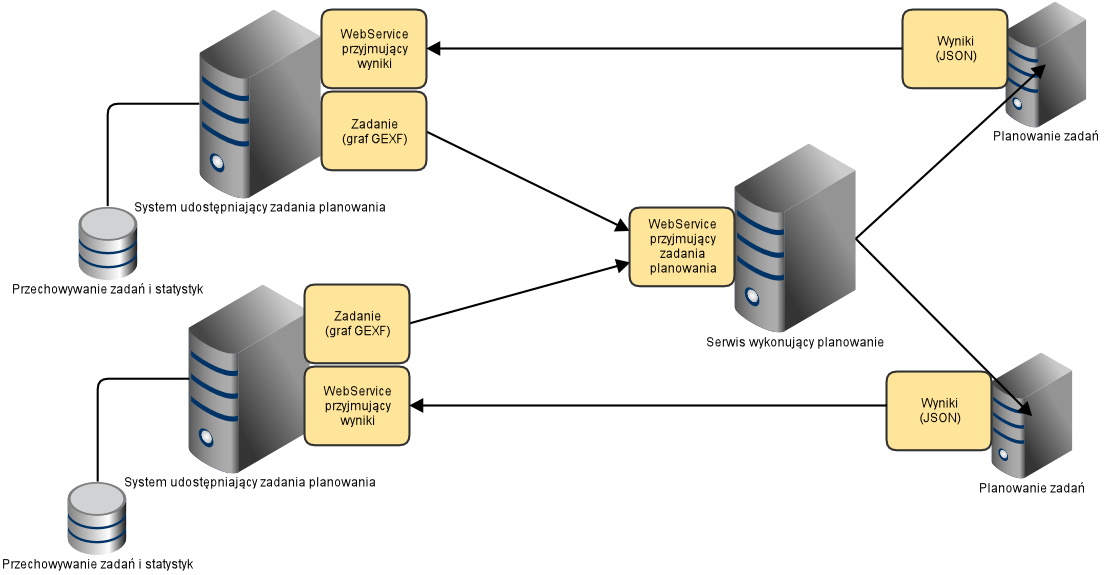
\includegraphics[width=\linewidth]{img/architektura}
	\caption{Architektura aplikacji.}
	\label{fig:architektura}
\end{figure}

\section{Web serwisy}
\label{sec:webservices}
\subsection{Web serwis przyjmujący zadania}

\subsection{Web serwis przyjmujący wyniki}

\section{Format danych}
\label{sec:data}

\subsection{GEXF}

\subsection{JSON}

\section{Algorytmy}

\subsection{BFS}

\subsection{DFS}

\subsection{A*}

\subsection{Bellman-Ford}

\subsection{Dijkstra}

\subsection{Uniform Cost}

\subsection{Floyd-Warshall}

\subsection{Prim}
aa

\subsection{Kruskal}

\section{Metryki}

\subsection{Czas wykonania}

\subsection{Zużycie pamięci}

\subsection{Waga ścieżki}

\section{Enterprise Integration Patterns}
W naszym projekcie wykorzystaliśmy cztery różne biblioteki do obliczeń grafowych. 
Każda z nich posiadała inną reprezentację danych. Wykorzystane biblioteki to:

\begin{itemize}
 \item JUNG
 \item GeoTools
 \item aima-java
 \item JGraphT
\end{itemize}

Aby umożliwić wykorzystanie algorytmów pochodzących z tych bibliotek, potrzebne było dokonanie transformacji przychodzących danych wejściowych z
formatu GEXF do formatu wykorzystywanego przez daną bibliotekę.
W tym celu skorzystaliśmy ze wzorców projektowych Enterprise Integration Patterns zaproponowanych w \cite{hohpe2004enterprise}.

\subsection{Normalizer}
Wzorzec projektowy Normalizer wykorzystuje Message Router aby skierować przychodzącą wiadomość do odpowiadającego jej Message Translatora.
Wymaga to, aby Message Router wykrył typ przesłanej wiadomości i na tej podstawie skierował ją w odopowienie miejsce.
Sytuacja została przedstawiona na rysunku \ref{fig:normalizer}

\begin{figure}[!h]
 \centering
 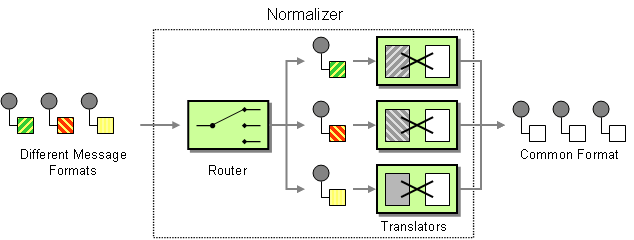
\includegraphics[width=1.0\textwidth]{eip/Normalizer}
 \caption{Wzorzec Normalizer}
 \label{fig:normalizer}
\end{figure}

\subsection{Message Router}
Worzec Message Router zapewnia przekazanie przychodzącej wiadomości do odpowiedniej kolejki w której odbędzie się dalsze przetwarzanie wiadomości.
Dokonuje się to, na podstawie wykrytego typu wiadomości.
Sytuacja została przedstawiona na rysunku \ref{fig:messageRouter}

\begin{figure}[!h]
 \centering
 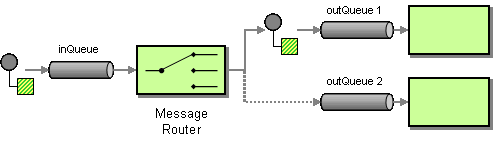
\includegraphics[width=1.0\textwidth]{eip/MessageRouter}
 \caption{Wzorzec Message Router}
 \label{fig:messageRouter}
\end{figure}

\subsection{Message Translator}
Wzorzec projektowy Message Translator wykorzystywany jest do transformacji przychodzącej wiadomości do określonego formatu wyjściowego.
Symbolicznie zostało to przedstawione na rysunku \ref{fig:messageTranslator}

\begin{figure}[!h]
 \centering
 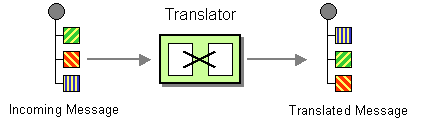
\includegraphics[width=1.0\textwidth]{eip/MessageTranslator}
 \caption{Wzorzec Message Translator}
 \label{fig:messageTranslator}
\end{figure}

\section{Uruchamianie zadań}
